% This work is licensed under the Creative Commons
% Attribution-NonCommercial 3.0 Unported License. To view a copy of this
% license, visit http://creativecommons.org/licenses/by-nc/3.0/.

\section{Auswertung}
\subsection{Bestimmung der Zeitkonstante}
\subsubsection{Mittels Entladevorgang}
Aus der Aufnahme des Spannungsverlaufes beim Entladevorgang des
Kondensators, welche in Abbildung~\ref{fig:aufnahme_zeitkonstante} zu
erkennen ist, werden die in Tabelle~\ref{tab:messwerte_zeitkonstante}
aufgeführten Werte abgelesen.
%
\begin{figure}
\centering
\includegraphics{zur_zeitkonstante}
\caption{Aufnahme eines Entladevorganges des Kondensators}
\label{fig:aufnahme_zeitkonstante}
\end{figure}
%
Ein Plot der logarithmisierten Spannungen gegen die Zeit, sowie die
Ausgleichsgerade durch diese Punkte ist in Abbildung
\ref{fig:zur_zeitkonstante} zu finden. Als Steigung m der
Ausgleichsgeraden ergibt sich ein Wert von
ca. \SI{-0.751(016)}{\per\milli\second}. Damit ergibt sich nach Formel
\eqref{eq:wert_rc}, die sich durch Äquivalenzumformungen aus Formel
\eqref{eq:sol-rc-dgl} ergibt, ein Wert für die Zeitkonstante $\tau$ von
\SI{1.331(029)}{\milli\second}.
\begin{equation}
\centering
\label{eq:wert_rc}
\tau = \frac{-1}{m}
\end{equation}
\begin{center}
m $\hat{=}$ Steigung der Ausgleichsgeraden
\end{center}
Der Fehler der Zeitkonstanten RC wird durch die in Formel \eqref{eq:gauss_zeitkonstante} angegebene Fehlerfortpflanzung errechnet.   
\begin{equation}
\centering
\label{eq:gauss_zeitkonstante}
\Delta \tau = \sqrt{ (\frac{\Delta m}{m^2})^2 }
\end{equation}
\begin{table}
  \centering
  \begin{tabular}{c|c}
    \toprule
    t in ms & $U_c$ in V\\
    \midrule
    0.0 &  11.7 \\
    0.5 &  8.3 \\
    1.0 &  5.7 \\
    1.5 &  4.0 \\
    2.0 &  2.8 \\
    2.5 &  2.0 \\
    3.0 &  1.3 \\
    3.5 &  0.8 \\
    \bottomrule
  \end{tabular}
  \caption{Messwerte beim Entladevorgang des Kondensators}
  \label{tab:messwerte_zeitkonstante}
\end{table}
\begin{figure}
\centering
\includegraphics{plot_zeitkonstante}
\caption{Messwerte zum Entladevorgang des Kondensators}
\label{fig:zur_zeitkonstante}
\end{figure}

\subsubsection{Mittels Amplitudenabnahme}
In Tabelle \ref{tab:messwerte_amplituden} sind die Werte der Amplitude
der Kondensatorspannung bei verschiedenen Frequenzen angegeben. Ein Plot
dieser Messwerte ist in Abb.~\ref{fig:plot_amplitude} zu finden. Es wird eine
nicht-lineare Ausgleichskurve durch die Messwerte gelegt, welche die in
Formel \eqref{eq:amplitude-frequenz} wiedergegebene Form hat. Die
Berechnung der optimalen Zeitkonstante $\tau$ wird über die Methode der
kleinsten Quadrate durchgeführt\footnote{Dazu wurde \texttt{ipython}
 in der Version 0.13  verwendet}. Als Ergebnis ergibt sich:
%
\begin{equation}
\tau_\text{neu} = \SI{1.372(001)}{\milli\second}
\end{equation}
%
Der in diesem Unterabschnitt bestimmte Wert für die Zeitkonstante $\tau$ unterscheidet sich also um \SI{0.041}{\milli\second}. Es ist zu beachten, dass bei dieser Messung der Innenwiderstand der Spannungsquelle, welcher in Reihe mit dem Widerstand des RC-Kreises geschaltet ist, die Messung beeinflusst. Es kann davon ausgegangen werden, dass sich dadurch der Gesamtwiederstand um \SI{600}{\ohm} erhöht. Der Vergleich der beiden bestimmten Zeitkonstanten ermöglicht es dadurch die Kapazität des verwendeten Kondensators zu berechnen.
\begin{equation*}
  \begin{split}
    \tau_\text{alt} + R_i C = \tau_\text{neu}\\
	\Leftrightarrow C = \frac{\tau_\text{neu} - \tau_\text{alt}}{R_i}
  \end{split}
\end{equation*}
\begin{table}
  \centering
  \begin{tabular}{c|c|c|c}
    \toprule
    v / Hz & A / V & v / Hz & A / V \\
    \midrule
     10 &3.86 &700 &0.621 \\
     20 & 3.86 &900 &0.486 \\
     40 &3.712 &1200& 0.365 \\
     60 &3.472 &1500& 0.292 \\
    100& 2.937 &1800& 0.243 \\
    150& 2.357 &2500& 0.175 \\
    200& 1.925 &3000& 0.145 \\
    300& 1.379 &4000& 0.109 \\
    400& 1.063 &5000& 0.087 \\
    500& 0.862 &10000& 0.031 \\ 
 \bottomrule
  \end{tabular}
  \caption{Messwerte der Amplitudenspannung bei verschiedenen Frequenzen}
  \label{tab:messwerte_amplituden}
\end{table}
\begin{figure}
  \centering
  \includegraphics{plot_amplitude}
  \caption{Amplitudenverlauf in Abhängigkeit der eingestellten Frequenz}
  \label{fig:plot_amplitude}
\end{figure}
Daraus ergibt sich eine Kapazität von C$\approx$\SI{68}{\nano\farad}
Mithilfe der Kapazität kann nun mit nachfolgender Rechnung der tatsächliche Wert der Zeitkonstante $\tau$ berechnet werden.
\begin{equation*}
  \begin{split}
    \tau + R_i C = \tau_\text{neu}\\
	\Leftrightarrow \tau = \tau_\text{neu} - R_i C
  \end{split}
\end{equation*}
Als tatsächlichen Wert für $\tau$ ergibt sich wieder ca. $\tau$ = \SI{1.372}{\milli\second} $\pm$ \SI{0.001}{\milli\second}.
\subsubsection{Mittels Phasenverschiebung}
In diesem Unterkapitel wird die Zeitkonstante $\tau$ mithilfe der wachsenden Phasendifferenz zwischen Spannungsquelle und Kondensator bei steigender Frequenz ermittelt.
Tabelle \ref{tab:messwerte_phase} enthält die gemessenen Werte für die
Zeitdifferenz zweier Nulldurchgänge zwischen Eingangsspannung und
Kondensatorspannung, die dazugehörigen Frequenzen und die Umrechnung der
Zeitdifferenzen in Phasendifferenzen. Die Umrechnung der Zeitdifferenzen
$\Delta t$ in Phasendifferenzen $\phi$ geschieht nach Formel
\eqref{eq:phase_zeit}.
%
\begin{equation}
  \label{eq:phase_zeit}
  \phi = 2 \pi \cdot \Delta t \cdot \nu
\end{equation}
%
\begin{table}
  \centering
  \begin{tabular}{c|c|c}
    \toprule
    v / Hz & $\Delta t$ / ms  & $\phi$ in Bogenmaß \\
    \midrule
     10 & 1680& 0.11 \\
     20 & 1500& 0.19\\
     40 & 1420& 0.36\\
     60 & 1360& 0.51\\
    100 & 1190& 0.75\\
    150 & 1000& 0.94\\
    200& 860& 1.08\\
    300 & 660& 1.24\\
    400 & 520& 1.31\\
    500 & 432& 1.36\\
    700 & 320& 1.41\\
    900 & 256& 1.45\\
   1200 & 196& 1.48\\
   1500 & 158& 1.49\\
   1800 & 133& 1.50\\
   2500 & 97& 1.52\\
   3000 & 81& 1.53\\
   4000 & 61& 1.53\\
   5000 & 49& 1.54\\
  10000 & 25& 1.58\\
 \bottomrule
  \end{tabular}
  \caption{Messwerte zur Phasendifferenz}
  \label{tab:messwerte_phase}
\end{table}
%
Die Messwerte sind als Plot in Abb.~\ref{fig:plot_phase} zu finden. Die
Ausgleichskurve besitzt die in Formel~\eqref{eq:phase_frequenz} angegebene
Form, wobei A die Amplitude und $U_0$ die eingestellte
Spannungsamplitude der Spannungsquelle bezeichnet. Der optimale
Parameter für $\tau$ wird mit \texttt{ipython} berechnet.
%
\begin{equation}
\label{eq:phase_frequenz}
\frac{A}{U_0}=cos{\phi}
\end{equation}
%
Das Ergebnis lautet nach dem Beachten des Innenwiderstandes der
Spannungsquelle:
\begin{equation*}
  \tau = \SI{1.482(001)}{\milli\second}
\end{equation*}
\begin{figure}
  \centering
  \includegraphics{plot_phase}
  \caption{Phasendifferenz in Abhängigkeit von der eingestellten Frequenz}
  \label{fig:plot_phase}
\end{figure}
Nun soll noch die Amplitude in Abhängigkeit von der Phasendifferenz in
einem Polarkoordinatensystem dargestellt werden. Die Messwerte sowie die
berechnete Kurve dieses Zusammenhangs kann man in
Abb.~\ref{fig:polarplot} erkennen. Dabei entspricht der Abstand eines
Punktes vom Mittelpunkt des Kreises dem Wert der Amplitude. Die
berechnete Kurve wird mithilfe von Formel~\eqref{eq:phase_frequenz}
bestimmt.
\begin{figure}
\centering
\includegraphics{polarplot}
\caption{Amplitudenhöhe gegen Phasendifferenz im Polarkoordinatensystem}
\label{fig:polarplot}
\end{figure}
\section{Der RC-Kreis als Integrator}
Wie im Theorieteil gezeigt,ist es möglich, einen RC-Kreis zum
Integrieren des Eingangssignals zu verwenden. Dazu wird eine hohe
Frequenz benötigt. In diesem Versuch wird die Frequenz auf
\SI{10000}{\hertz} eingestellt. Bei der Betrachtung der Abbildungen
\ref{fig:integration_rechteck}, \ref{fig:integration_sinus} und
\ref{fig:integration_dreieck} sind die Eingangs- und Ausgangssignale des
RC-Kreises bei genanntet Frequenz zu erkennen. Dabei befindet sich das
Eingangssignal in den Abbildungen immer oben und das Ausgangssignal
unten.

\begin{figure}
  \centering
  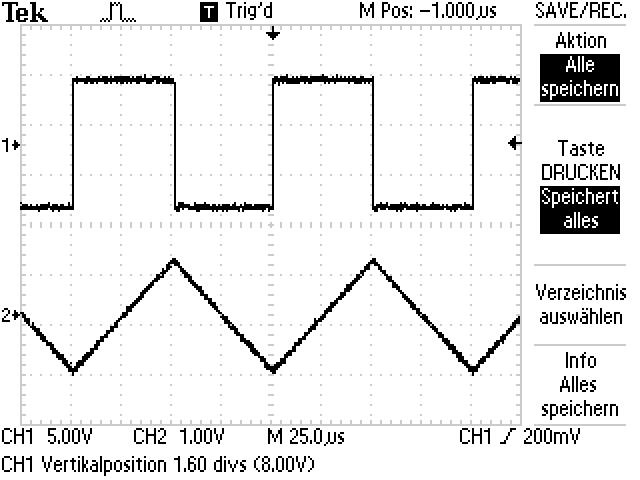
\includegraphics{integration_rechteck}
  \caption{Integration des Rechtecksignals}
  \label{fig:integration_rechteck}
\end{figure}

\begin{figure}
  \centering
  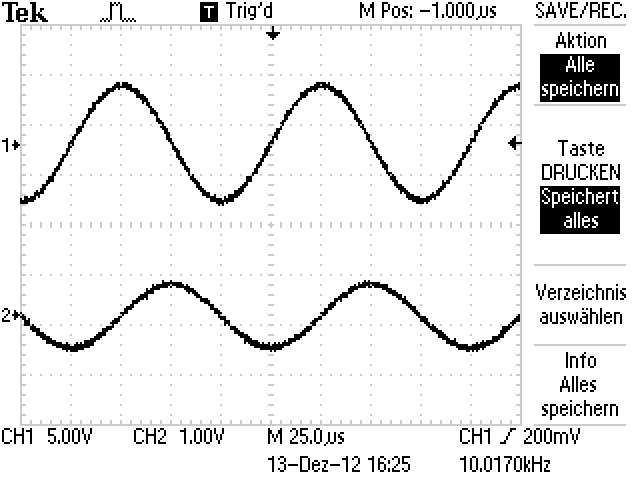
\includegraphics{integration_sinus}
  \caption{Integration des Sinussignals}
  \label{fig:integration_sinus}
\end{figure}

\begin{figure}
  \centering
  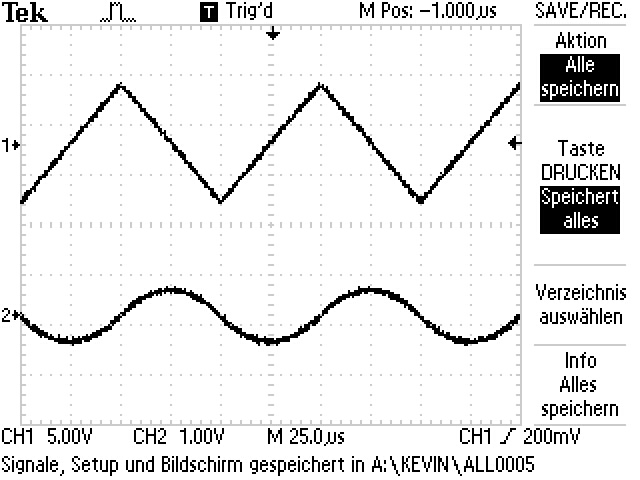
\includegraphics{integration_dreieck}
  \caption{Integration des Dreiecksignals}
  \label{fig:integration_dreieck}
\end{figure}
